\subsubsection{Detaillierte Implementation}

Eine Übersicht der einzelnen Komponenten mit ihren genauen Zusammenhängen wird in Abbildung~\ref{asset:Capacitor-BrowserView:Implementation} dargestellt.

\begin{figure}[H]
    \centering
    \vspace{1em}
    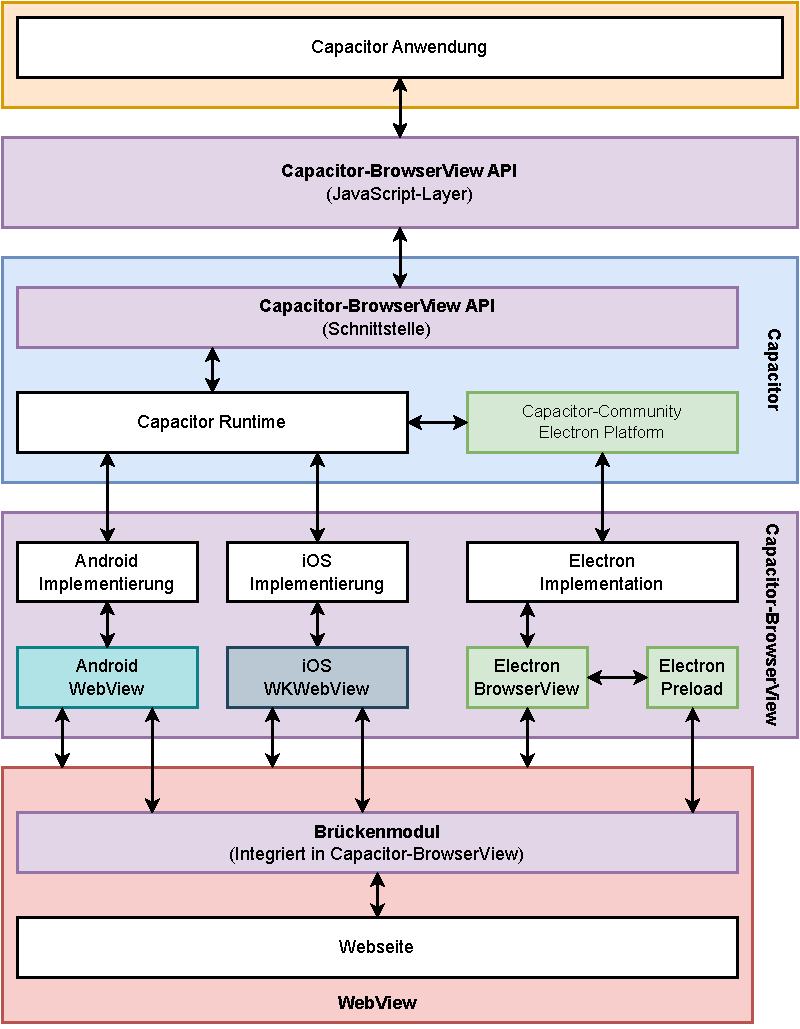
\includegraphics[width=\textwidth]{assets/03_Capacitor-BrowserView/03_Implementation.drawio.pdf}
    \caption[Capacitor-BrowserView / Implementierung]{Implementierung des Capacitor-BrowserView Plugins}
    \label{asset:Capacitor-BrowserView:Implementation}
\end{figure}

\newpage

\paragraph{Plugin API}

Das Capacitor-BrowserView Plugin erweitert seine \ac{api} um einen zusätzlichen JavaScript"=Layer, der zusätzliche nicht-native Funktionen implementiert.
Damit wird das Entfernen bestimmter oder aller Event-Listener sowie das Erstellen von \enquote{BrowserView}"=Instanzen ermöglicht.

Um die Erstellung von \enquote{BrowserView}"=Instanzen zu ermöglichen, wird die ursprüngliche Plugin \ac{api} in eine Klasse gekapselt.
BrowserViews können dadurch einfach über eine Instanz dieser Klasse erstellt werden.
Dies vereinfacht die Verwendung der Plugin \ac{api} wesentlich, da Methoden für eine bestimmte BrowserView direkt von der entsprechenden Instanz ausgeführt werden können.
Anderenfalls müssten die Methoden mit der entsprechenden \ac{uuid} der BrowserView aufgerufen werden.

Ein weiterer Vorteil dieser Umsetzung ist eine Reduzierung der Fehleranfälligkeit, da die \acp{uuid} der verwendeten BrowserViews nicht manuell verwaltet werden müssen.

\newpage

\paragraph{Implementierungen}

Um die Implementierung des Plugins auf allen Plattformen übersichtlich und wartungsfreundlich zu gestalten, sind sie in ihrer Struktur sehr ähnlich.
Sie bestehen jeweils aus zwei Teilen:

\begin{enumerate}
    \item 
    Der erste Teil wird von der Capacitor Runtime aufgerufen.
    Er implementiert die \acs{api}-Struktur und wertet die Parameter der Methoden aus.
    \item
    Der zweite Teil implementiert die tatsächlichen Funktionen, wie das Erstellen und Steuern von WebViews
    sowie das Senden und Empfangen von Nachrichten zwischen der Capacitor Anwendung und den geladenen Webinhalten.
\end{enumerate}

Für die Implementierung des Plugins wurden ausschließlich die jeweiligen Plattform"=\acsp{api} verwendet, da WebViews auf jeder Plattform nativ unterstützt werden.
\cite{android:api, ios:api, electron:docs}

Die WebView \acsp{api} sind auf den verschiedenen Plattformen nicht vollständig identisch.~\cite{android:api, electron:docs}
Daher musste für die Implementierung des Plugins ein Kompromiss gefunden werden, um die angestrebte Wartungsfreundlichkeit zu realisieren.
Einige fehlende Funktionen wurden im Plugin nachgebaut, und einige Funktionen werden aufgrund großer Unterschiede nicht unterstützt.

\begin{itemize}
    \setlength\itemsep{-0.5em}
    \item
    Um die Position einer WebViews unter Android festzulegen, muss die Pixeldichte des Geräts berücksichtigt werden.
    Andernfalls stimmen die Koordinaten und Abmessungen der WebView nicht mit der Capacitor Anwendung überein.
    Auch die Höhe der Statusleiste von Android muss berücksichtigt werden, da sich die WebView sonst mit ihr überschneiden würde.
    Die von Electron unter Windows, Linux und macOS bereitgestellte BrowserView führt diese erforderlichen Umrechnungen selbständig durch.
    \item
    Die Android WebView bietet eine Einstellung, um das Öffnen von Webinhalten in einem neuen Fenster über Web \acp{api} zu erlauben oder zu verbieten.~\cite{android:api}
    Diese Einstellung ist in Electron unter Windows, Linux und macOS nicht direkt in dieser Form verfügbar.~\cite{electron:docs}
    Daher wurde sie in das Plugin nachträglich für Electron implementiert.
    \item
    Favicons, kleine Symbole für das Branding von Webinhalten, werden in der Android WebView direkt in einem Binärformat bereitgestellt,
    während unter Windows, Linux und macO in Electron nur der Link zum Symbol bereitgestellt wird.~\cite{android:api, electron:docs}
    Daher wird es vom Plugin nachträglich heruntergeladen.
    Um das Symbol über die Plugin \ac{api} leicht zugänglich zu machen, wird es zudem vom Plugin mit Base64 in eine Zeichenkette kodiert
    \item
    Android WebViews unterstützen standardmäßig keinen Vollbildmodus.
    Daher wurde diese Funktion nachträglich in das Plugin implementiert.
    Notwendige Parameter für einen vollständigen Vollbildmodus in einer Android App wurden von StackOverflow bezogen.
    \cite{android:api, stackoverflow}
\end{itemize}

\newpage

\paragraph{Interprozesskommunikation}

Standardmäßig ist die Kommunikation zwischen Webinhalten und der Capacitor-Anwendung deaktiviert.
Dies dient der Isolation von möglichen unsicheren Inhalten.
Wenn jedoch ein vertrauenswürdiger Inhalt geladen wird, mit dem ein Datenaustausch erforderlich ist, wird dennoch eine Interprozesskommunikation vom Plugin bereitgestellt.

Um die Kommunikation zwischen vertrauenswürdigen Webinhalten, der Plugin Implementierung und der Capacitor Anwendung zu ermöglichen, wird unter Android die \code{addJavascriptInterface}"=\acs{api} der WebView verwendet.
Diese \ac{api} ermöglicht es, eine Java-Funktion in die Webseite einzuspeisen.~\cite{android:api}

Für Windows, Linux und macOS wurde unter Electron für ein ähnliches Verhalten das Preload-Skript mit der \code{contextBridge}"=\acs{api} verwendet.
Diese \ac{api} ermöglicht es ebenfalls, eine Funktion in die Webseite einzuspeisen.~\cite{electron:docs}

Die eingespeiste Funktion dient als Schnittstelle, um Daten von der geladenen Webseite an das Capacitor-BrowserView Plugin zu senden.
Das Plugin leitet dann die empfangenen Daten an die Capacitor Anwendung weiter.

Um Daten von der Capacitor Anwendung an die Webseite zu senden, verwendet das Plugin die \code{evaluateJavascript}"=Methode der Android WebView bzw.\ die \code{executeJavaScript}"=Methode der Electron BrowserView unter Windows, Linux und macOS\@.
Dadurch kann ein JavaScript-Code auf der Webseite ausgeführt werden~\cite{android:api, electron:docs}, der die Daten über die \code{dispatchEvent} Web-\acs{api} an die entsprechenden Event-Listener auf der Webseite verteilt.~\cite{web:api}

Unter Android können Nutzdaten nur als primitive Datentypen übergeben werden \cite{android:api}, daher müssen diese Daten Serialisiert und Deserialisiert werden.
Für die Serialisierung wurde das \ac{json} Datenformat verwendet.

Zur Verbesserung der Benutzerfreundlichkeit wurde ein Brückenmodul entwickelt, welches eine vereinfachte \ac{api} für die Kommunikation zur Capacitor Anwendung auf der Webseite bereitstellt.
Das Modul übernimmt den Zugriff auf die eingespeiste Funktion \textit{(um Daten zu senden)}, die Registrierung von Event-Listener \textit{(um Daten zu empfangen)} sowie die Serialisierung und Deserialisierung der Nutzdaten.

Um das automatische Laden des Brückenmoduls zu ermöglichen, wird das Modul beim Start des Ladevorgangs der Webseite ausgeführt.

Unter Windows, Linux und macOS bzw.\ unter Electron ist das Ausführen des Moduls jedoch erst erlaubt, wenn die Webseite vollständig geladen wurde.
Folglich könnte die Webseite nicht rechtzeitig auf die \ac{api} des Brückenmoduls zugreifen.
Um dennoch das rechtzeitige Laden des Moduls zu ermöglichen, wird das Electron Preload-Skript mit der \code{contextBridge}"=\acs{api} verwendet.
\cite{electron:docs}
